%$Id: chi06.tex,v 1.4 2006/02/13 23:19:21 rlw Exp rlw $
%\documentclass[]{beamer}
\documentclass[handout]{beamer}
%\usetheme[hideothersubsections]{PaloAlto}
\usepackage{comment,auto-pst-pdf}
\usepackage{amsmath,amssymb,bm,array,graphicx,epic,psfrag}
\usepackage{multirow, dcolumn}
%\usepackage{movie15}
%\bibliographystyle{jasa}
\graphicspath{{./}{eps/}}
\setbeamercovered{transparent}
\title{Bayesian Adpative Regression Kernels \& SVM}
\author[M. Clyde]{Merlise Clyde}
\institute{Department of Statistical Science \\ Duke
University }
\date{\today}
\newcommand{\bs}[2]{\begin{frame} \frametitle{#1}
{#2}
\end{frame} }
\usepackage{xcolor}
\definecolor{beamer@blendedblue}{RGB}{86,155,189}
\definecolor{myblue}{RGB}{12,76,138}
\setbeamercolor{structure}{fg=myblue}
\definecolor{Ftitle}{RGB}{12,76,138}
\definecolor{Descitem}{RGB}{238,238,244}
\definecolor{StdTitle}{RGB}{12,76,138}
\definecolor{StdBody}{RGB}{213,24,0}
\definecolor{StdBody}{RGB}{213,24,0}

\definecolor{AlTitle}{RGB}{255, 190, 190}
\definecolor{AlBody}{RGB}{213,24,0}

\definecolor{ExTitle}{RGB}{201, 217, 217}
\definecolor{ExBody}{RGB}{213,24,0}

\setbeamercolor{frametitle}{fg = Ftitle}
\setbeamercolor{title}{fg = Ftitle}
\setbeamercolor{item}{fg = Ftitle}
\setbeamercolor{subitem}{fg = Ftitle}
\setbeamercolor{subsubitem}{fg = Ftitle}
\setbeamercolor{description item}{fg = myblue}
\setbeamercolor{titlelike}{fg=myblue}

\DeclareMathOperator{\sgn}{sgn}
\newcommand{\e}{\mathbf{e}}
\renewcommand{\P}{\mathbf{P}}
\newcommand{\F}{\mathbf{F}}
\newcommand{\R}{\textsf{R}}
\newcommand{\mat}[1] {\mathbf{#1}}
%\newcommand{\ind}{\mathrel{\mathop{\sim}\limits^{\mathit{ind}}}}
%\newcommand{\iid}{\mathrel{\mathop{\sim}\limits^{\mathit{iid}}}}
\newcommand{\E}{\textsf{E}}
\newcommand{\SE}{\textsf{SE}}
\newcommand{\SSE}{\textsf{SSE}}
\newcommand{\RSS}{\textsf{RSS}}
\newcommand{\FSS}{\textsf{FSS}}
\renewcommand{\SS}{\textsf{SS}}
\newcommand{\MSE}{\textsf{MSE}}
\newcommand{\SSR}{\textsf{SSR}}
\newcommand{\Be}{\textsf{Beta}}
\newcommand{\St}{\textsf{St}}
\newcommand{\Ca}{\textsf{C}}
\newcommand{\Exp}{\textsf{Exp}}
\newcommand{\GDP}{\textsf{GDP}}
\newcommand{\NcSt}{\textsf{NcSt}}
\newcommand{\Bin}{\textsf{Bin}}
\newcommand{\NB}{\textsf{NegBin}}
\renewcommand{\NG}{\textsf{NG}}
\newcommand{\N}{\textsf{N}}
\newcommand{\Ber}{\textsf{Ber}}
\newcommand{\Poi}{\text{Poi}}
\newcommand{\Gam}{\textsf{Gamma}}
\newcommand{\BB}{\textsf{BB}}
\newcommand{\Gm}{\textsf{G}}
\newcommand{\Un}{\textsf{Unif}}
\newcommand{\Ex}{\textsf{Exp}}
\newcommand{\DE}{\textsf{DE}}
\newcommand{\tr}{\textsf{tr}}
\newcommand{\cF}{{\cal{F}}}
\newcommand{\cL}{{\cal{L}}}
\newcommand{\cI}{{\cal{I}}}
\newcommand{\cB}{{\cal{B}}}
\newcommand{\cP}{{\cal{P}}}
\newcommand{\bbR}{\mathbb{R}}
\newcommand{\bbN}{\mathbb{N}}
\newcommand{\pperp}{\mathrel{{\rlap{$\,\perp$}\perp\,\,}}}
\newcommand{\OFP}{(\Omega,\cF, \P)}
\newcommand{\eps}{\boldsymbol{\epsilon}}
\newcommand{\1}{\mathbf{1}_n}
\newcommand{\gap}{\vspace{8mm}}
\newcommand{\ind}{\mathrel{\mathop{\sim}\limits^{\rm ind}}}
\newcommand{\simiid}{\ensuremath{\mathrel{\mathop{\sim}\limits^{\rm
iid}}}}
\newcommand{\eqindis}{\ensuremath{\mathrel{\mathop{=}\limits^{\rm D}}}}
\newcommand{\iid}{\textit{i.i.d.}}
\newcommand{\SSZ}{S_{zz}}
\newcommand{\SZW}{S_{zw}}
\newcommand{\Var}{\textsf{Var}}
\newcommand{\corr}{\textsf{corr}}
\newcommand{\diag}{\textsf{diag}}
\newcommand{\var}{\textsf{var}}
\newcommand{\Cov}{\textsf{Cov}}
\newcommand{\Sam}{{\cal S}}
\def\H{\mathbf{H}}
\newcommand{\I}{\mathbf{I}}
\newcommand{\Y}{\mathbf{Y}}
\newcommand{\tY}{\tilde{\mathbf{Y}}}
\newcommand{\Yhat}{\hat{\mathbf{Y}}}
\newcommand{\Yobs}{\mathbf{Y}_{{\cal S}}}
\newcommand{\barYobs}{\bar{Y}_{{\cal S}}}
\newcommand{\barYmiss}{\bar{Y}_{{\cal S}^c}}
\def\bv{\mathbf{b}}
\def\X{\mathbf{X}}
\def\tX{\tilde{\mathbf{X}}}
\def\x{\mathbf{x}}
\def\xbar{\bar{\mathbf{x}}}
\def\Xbar{\bar{\mathbf{X}}}
\def\Xg{\mathbf{X}_{\boldsymbol{\gamma}}}
\def\Ybar{\bar{\Y}}
\def\ybar{\bar{y}}
\def\y{\mathbf{y}}
\def\Yf{\mathbf{Y_f}}
\def\W{\mathbf{W}}
\def\L{\mathbf{L}}
\def\w{\mathbf{w}}
\def\U{\mathbf{U}}
\def\V{\mathbf{V}}
\def\Q{\mathbf{Q}}
\def\Z{\mathbf{Z}}
\def\z{\mathbf{z}}
\def\v{\mathbf{v}}
\def\u{\mathbf{u}}

\def\zero{\mathbf{0}}
\newcommand{\one}{\mathbf{1}}
\newcommand{\taub}{\boldsymbol{\tau}}
\newcommand{\betav}{\boldsymbol{\beta}}
\newcommand{\alphav}{\boldsymbol{\alpha}}
\newcommand{\A}{\mathbf{A}}
\def\a{\mathbf{a}}
\def\K{\mathbf{K}}
\newcommand{\B}{\mathbf{B}}
\def\b{\boldsymbol{\beta}}
\def\bhat{\hat{\boldsymbol{\beta}}}
\def\btilde{\tilde{\boldsymbol{\beta}}}
\def\tb{\boldsymbol{\theta}}
\def\bg{\boldsymbol{\beta_\gamma}}
\def\bgnot{\boldsymbol{\beta_{(-\gamma)}}}
\def\mub{\boldsymbol{\mu}}
\def\tmub{\tilde{\boldsymbol{\mu}}}
\def\muhat{\hat{\boldsymbol{\mu}}}
\def\tb{\boldsymbol{\theta}}
\def\tk{\boldsymbol{\theta}_k}
\def\tj{\boldsymbol{\theta}_j}
\def\Mk{\boldsymbol{{\cal M}}_k}
\def\M{\boldsymbol{{\cal M}}}
\def\Mj{\boldsymbol{{\cal M}}_j}
\def\Mi{\boldsymbol{{\cal M}}_i}
\def\Mg{{\boldsymbol{{\cal M}_\gamma}}}
\def\Mnull{\boldsymbol{{\cal M}}_{N}}
\def\gMPM{\boldsymbol{\gamma}_{\text{MPM}}}
\def\gHPM{\boldsymbol{\gamma}_{\text{HPM}}}
\def\Mfull{\boldsymbol{{\cal M}}_{F}}
\def\tg{\boldsymbol{\theta}_{\boldsymbol{\gamma}}}
\def\g{\boldsymbol{\gamma}}
\def\eg{\boldsymbol{\eta}_{\boldsymbol{\gamma}}}
\def\G{\mathbf{G}}
\def\cM{\cal M}
\def\D{\Delta}
\def \shat{{\hat{\sigma}}^2}
\def\uv{\mathbf{u}}
\def\l {\lambda}
\def\d{\delta}
\def\Sigmab{\boldsymbol{\Sigma}}
\def\Lambdab{\boldsymbol{\Lambda}}
\def\lambdab{\boldsymbol{\lambda}}
\def\Mg{{\cal M}_\gamma}
\def\S{{\cal{S}}}
\def\qg{p_{\boldsymbol{\gamma}}}
\def\pg{p_{\boldsymbol{\gamma}}}
%\def\t{\mathbf{t}}
\def\T{\boldsymbol{\Theta}}
\def\Tb{\boldsymbol{\Theta}}



\begin{document}
\begin{frame}
  \titlepage
\end{frame}

\section{Motivation}

\subsection{Mass Spectroscopy}
\bs{MALDI-TOF Mass Spectroscopy} {
\centerline{  \includegraphics[height=2in]{mean-spectrum.ps}}

%\vspace{-.25in}
Location of peaks/proteins in spectra  in the presence of noise

Non-Gaussian  Noise
%Deconvolution problem
}


\bs{Multiple Spectra} {
\begin{center}
\begin{tabular}{cc}
\includegraphics[height=1in,angle=-90]{RawSpecCont_n4_allFrcAvg_22.ps}&
\includegraphics[height=1in,angle=-90]{RawSpecDis_n15_allFrcAvg_22.ps}\vspace{-.2in}\\
\includegraphics[height=1in,angle=-90]{RawSpecCont_n2_allFrcAvg_22.ps}&
\includegraphics[height=1in,angle=-90]{RawSpecDis_n14_allFrcAvg_22.ps}\vspace{-.2in}\\
\includegraphics[height=1in,angle=-90]{RawSpecCont_n1_allFrcAvg_22.ps}&
\includegraphics[height=1in,angle=-90]{RawSpecDis_n11_allFrcAvg_22.ps}
%\includegraphics[angle=-90]{/proj/levy/proteomics/multiSpec_paper/paper_figures/RawSpecCont_Frc5_subset.ps}&
%\includegraphics[angle=-90]{/proj/levy/proteomics/multiSpec_paper/paper_figures/RawSpecDis_Frc5_subset.ps}\\
\end{tabular}
\end{center}

Learning ``features'' that are common versus those that separate
groups of  spectra but do not know a prior the number of ions
}


\section{Nonparametric Regression}

\bs{Problem Setting}{
Regression problem
$$ \E[Y \mid \bfx] = f(\bfx), \quad \bfx \in \cfX$$
with unknown function $f(\bfx): \cfX \to \bbR$ \pause


\vspace{.5in}
Nonparametric Bayesian would place  prior distribution on functions


}

\subsection{Stochastic Expansions}
\bs{Expansions} {

Write function as
 $$f(\bfx_i) = \sum_{j=0}^{J}  \psi(\bfx_i, \bfomega_j)\beta_j$$ in
terms of an (over-complete) dictionary where \pause

  \begin{itemize}
   \item  $\{\beta_j\}$:  unknown coefficients \pause
   \item  $J$: number of terms in expansion (finite or infinite) \pause


 \item $\psi(\bfx,\bfomega_j)$   Dictionary elements from
a ``generator function'' $g$ \pause
  \begin{itemize}
  \item cubic splines
$$   \psi(x_i, \omega_j) =  (x_i - \omega_j)^3_+$$ \pause
  \item multivariate kernels  (Gaussian, Cauchy, Exponential, e.g.)
$$  \psi(\bfx_i, \bfomega_j) =  g(
\bfLambda_j (\bfx - \mean_j)) = \exp\left\{-\frac{1}{2}(\bfx - \mean_j)^T \bfLambda_j (\bfx -
  \mean_j)\right\}$$  \pause
  \item translation and scaling wavelet families  \pause

\item Need not be symmetric!
  \end{itemize}
  \end{itemize}


}


\bs{Kernel Convolution } {
    \includegraphics[angle=270,origin=l,totalheight=6truecm,
     clip=1, width=10cm]{gammaproc2.ps}

Easy to generate  non-stationarity processes

}







\bs{Bayesian NonParametrics}{
Goal: $f(x) = \sum_{j < J}  \psi(\bfx, \bfomega_j) \beta_j = \sum_{j <
  J} g(\Scale_j(\bfx - \mean_j)) \beta_j$
\pause


\pause

\begin{itemize}
\item Poisson prior on $J$  (could be infinite!)
\item[$\Rightarrow$] $J \sim \Po(\nu_+)$,\qquad $\nu_+\equiv
  \nu(\bbR\times\bfOmega) = \iint v(\beta, \bfomega) d \beta \,
  d\bfomega$  \pause
\item[$\Rightarrow$] $\beta_j,\bfomega_j \mid J \iid \pi(\beta, \bfomega)
  \propto \nu(\beta,\bfomega)$. \pause
\end{itemize}

\begin{itemize}
  \item Finite number of ``big'' coefficients $|\beta_j|$ \pause
  \item Possibly infinite number of $\beta \in [-\epsilon, \epsilon]$ \pause
  \item Coefficients $|\beta_j|$ are absolutely summable \pause
 \end{itemize}

{Sufficient condition} for bounded $\k$:
\begin{equation}
  \label{eq:l1-bound}
\int_{\bbR \times \Omega} \min(1, |\beta|) \nu(\beta,
  \bfomega)d \beta \,
  d\bfomega  < \infty
\end{equation}


}


\bs{$\alpha$-Stable L\'evy Measures} {

L\'evy measure: $\nu(\beta, \bfomega) =  c_\alpha |\beta|^{-(\alpha
    +1)}\ \pi(\bfomega) \qquad 0 < \alpha < 2$ \pause

For $\alpha$- Stable $\nu^+(\bbR, \bfOmega) = \infty$ \pause

Fine in theory, but not in practice for MCMC! \pause

\vspace{14pt}
Truncate measure to obtain a finite expansion:
\begin{itemize}
 \item Finite number of support points $\bfomega$ with $\beta$ in
   $[-\epsilon, \epsilon]^c$  \pause
\item Fix $\epsilon$  (for given prior approximation error) \pause
\item Use approximate L\'evy  measure
$\nu_{\epsilon}(\beta, \bfomega) \equiv \nu(\beta,
\bfomega)\bfone(|\beta| > \epsilon) $ \pause
\item[$\Rightarrow$] $J \sim \Po(\nu_{\epsilon}^+)$ where
  $\nu^+_{\epsilon} = \nu([-\epsilon, \epsilon]^c, \bfOmega)$ \pause
\item[$\Rightarrow$]  $\beta_j, \bfomega_j \iid \pi(d\beta, d\bfomega) \equiv
  \nu_\epsilon(d\beta , d \bfomega)/\nu^+_{\epsilon}$ ($\beta_j$
  distributed as Pareto)

\end{itemize}
}


\bs{Truncated Cauchy Process} {
\centerline{Restriction  $|\beta| > \epsilon$}

%\psfrag{x}{\small{$\beta$}}
\centerline{\includegraphics[width=2.5in,angle=270]{cauchy1.ps}}
}


\bs{Contours of Log Prior (in $\bbR^2$) -- Penalties} {
\begin{tabular}{ccc}
Normal  & DE  & Cauchy \\
\includegraphics[angle=270,width=1.25in]{L2.ps} &
\includegraphics[angle=270,width=1.25in]{L1.ps} &
\includegraphics[angle=270,width=1.25in]{cauchy.ps}
\end{tabular}

\vspace{.25in}
Penalized Likelihood:
$$-\frac{1}{2 \sigma^2} \sum_i\left(Y_i - f(\bfx_i)\right)^2  - (\alpha +
1) \sum_j
\log(|\beta_j|)  - \nu^+_{\epsilon} \ldots $$

}




\bs{Computation - Reversible Jump MCMC} {

  \begin{itemize}
  \item Birth: generate coefficients $\beta_j$ near $\eps$ in absolute value
    and generate kernel parameters $\bfomega_j$ given increase in $J
    \to J+1$ \pause
\item Death: $\beta_j = 0$  drop dictionary element when $J$
  decrements by $1$.  \pause
\item Update:  Random-Walk update, but also leads to deaths with
  coefficients that wander out of bounds and cross $\eps$
  boundary! \pause
\item Merge-Split: allow ``neighboring points'' to merge into one
  dictionary element (an alternative death) or a split into  new
  dictionary elements \pause
  \end{itemize}
Advantage over fixed dimensional over-complete methods (frames)

}


\bs{Wavelet Test Functions (SNR = 7)} {
\begin{figure}[!h]
  \begin{center}
    \includegraphics[angle=270,origin=l,totalheight=6truecm,
     clip=1,width=10cm]{wavedata.ps}
  \end{center}
\end{figure}
}

\bs{Kernel Functions}{
\begin{figure}[!h]
  \begin{center}
    \includegraphics[angle=270,origin=l,totalheight=6truecm,
     clip=1,width=10cm]{kerplot.ps}
  \end{center}
\end{figure}
}

\bs{Comparisons of OCD Methods} {
  \begin{itemize}
  \item Translational Invariant Wavelets -- Laplace Priors
    (Johnstone \& Silverman     2005)
  \item Continuous Wavelet Dictionary -- Compound Poisson with
    Gaussian Priors (Chu, Clyde, Liang 2007)
  \item LARK Symmetric Gamma
  \item LARK Cauchy
  \end{itemize}
Range of Over-complete Dictionaries and Priors
}
\bs{Comparison of Mean Square Error w/ OCDs} {
100 realizations of each function

\centerline{\includegraphics[width=2.5in,angle=270]{mse.eps} }
}
%\subsection{Motorcycle Crash Data}
\bs{ Motorcycle Crash Data: A Real Example}{
On average, only $\E[J\mid Y]\approx 4$ jumps are needed for fit:\par
    \includegraphics[angle=270,origin=l, clip=1,
     totalheight=6truecm,width=10cm]{motorfitted.ps}
}

\bs{Form of Kernel} {
\[k(t_i; \tau_j, \lambda_j) = e^{-\lambda_j |t_i - \tau_j|^\rho}\]

    \includegraphics[angle=270,origin=l, clip=1,
     totalheight=6truecm,width=10cm]{motor-rho.ps}
}


\subsection{Moving to Higher Dimensions}


\bs{Higher Dimensional $\cfX$} {

RJ-MCMC is (currently) too slow in higher dimensional space to allow \pause
\begin{itemize}
\item $\bfchi$ to be completely arbitrary; restrict support to
  observed $\{\bfx_i\}$ like in SVM \pause
\item use diagonal $\bfLambda$
\end{itemize}
Kernels take form:
\begin{eqnarray*}
\psi(\bfx, \bfomega_j) & = & \prod_d \exp\{ -\frac{1}{2} \lambda_d (x_d - \chi_{d})^2
\} \\
f(\bfx) & =  & \sum_j \psi(\bfx, \bfomega_j) \beta_j
\end{eqnarray*}
}


\bs{Approximate L\'evy Prior II} {
Continuous Approximation Student $t(\alpha, 0, \epsilon)$ approximation:

$$\nu_\epsilon(d\beta, d \bfomega) = c_\alpha (\beta^2 + \alpha
\epsilon^2)^{-(\alpha + 1)/2} d\beta \ \gamma(d \bfomega) $$

\pause

Based on the following hierarchical prior
\begin{eqnarray*}
  \beta_j \mid \phi_j & \ind & \No(0,  \varphi_j^{-1}) \\
  \phi_j    & \ind & \Ga\left(\frac{\alpha}{2}, \frac{\alpha \epsilon^2}{2}\right) \\
   J & \sim & \Po(\nu^+_\epsilon)
\end{eqnarray*}

where $\nu^+_\epsilon = \nu_\epsilon(\bbR, \bfOmega) = \frac{\alpha ^{1
    - \alpha/2} \Gamma(\alpha)\Gamma(\alpha/2)}{\epsilon^\alpha
  \pi^{1/2} \Gamma(\frac{\alpha +1}{2})} \sin(\frac{\pi \alpha} {2}) \gamma(\bfOmega)$

Key:  need to have variance of coefficients decrease as $J$ increases
}

\bs{Limiting Case} {
  \begin{eqnarray*}
    \beta_j   \mid  \varphi_j & \ind &\N(0, 1/\varphi_j) \\
      \varphi_j & \iid & \Ga(\alpha/2, "0")
  \end{eqnarray*}
\pause

Notes:
  \begin{itemize}
\item Require $0 < \alpha < 2$  Additional restrictions  on $\omega$  \pause
\item  Cauchy process corresponds to $\alpha = 1$ \pause
\item  Tipping's ``Relevance Vector Machine'' corresponds to $\alpha =
  0$  (improper posterior!) \pause
\item Provides an extension of {\bf{Generalized Ridge Priors}}
      to infinite dimensional case \pause
\item Infinite dimensional analog of Cauchy priors
 \end{itemize}
}

\bs{Further Simplification in Case with $\alpha = 1$} {
  \begin{itemize}
  \item Poisson number of points $J_\eps\sim \Po\big(
    \nu_\eps^+(\alpha, \gamma) \big)$ with $\nu_\eps^+(\alpha, \gamma)
  = \frac{\gamma \alpha^{1-\alpha/2}}{2^{1 - \alpha}\eps^\alpha}
  \frac{\Gamma(\alpha/2)}{\Gamma(1-\alpha/2)}$ \pause
  \item Given $J$, $[ n_1 : n_n] \sim  MN(J, 1/(n+1))$ points
    supported at each kernel located at $\bfx_j$  \pause
  \end{itemize}
The regression mean function can be rewritten as
\[
  f(\bfx) = \sum_{i=0}^n \tilde{\beta}_i \psi(\bfx, \bfomega_i), \quad
  \tilde{\beta}_i = \sum_{\{j \, \mid \bfchi_j = \bfx_i\}} \beta_j.
\]
\pause
In particular, if $\alpha = 1$, not only the Cauchy process is infinitely
divisible, the approximated Cauchy prior distributions on the regression
coefficients are also infinitely divisible:

$$
  \tilde{\beta}_i  \ind
  \No(0, n_i^2 \tilde{\varphi}_i^{-1}), \qquad
  \tilde{\varphi}_i \iid \Ga( 1/2, \eps^2/2)
$$
\pause
At most $n$ non-zero coefficients!    (JAGS is possible now?)
}

\bs{Collapsed Sampler} {

{\bf Advantage}: Gaussian prior so $\beta$ can be integrated out for MCMC
under Gaussian error model in the $n$ dimensional problem \pause

\begin{itemize}
\item Integrate out $\beta$ vector in Normal regression leaving kernel
  parameters $\bfLambda$ and $\varphi$ with multinomial weights $n_i$  \pause
\item $n_i$ may be 0 which drops dictionary elements from
  representation in finite representation for fixed $\epsilon$ \pause

\item still trans-dimensional in $\varphi$ but much simpler RJMCMC now
\end{itemize}
}

\bs{Feature Selection in Kernel} {
\begin{itemize}
\item Product structure allows interactions between variables  \pause
\item Many input variables may be irrelevant \pause
\item Feature selection; if $\lambda_d = 0$ variable $x_d$ is removed
  from all kernels \pause
\item Allow point mass on $\lambda_h = 0$ with probability $p_\lambda
  \sim B(a,b)$  (in practice have used $a = b = 1$ \pause
\end{itemize}

Consider 3 Scenarios

\begin{itemize}
\item $D$ Different $\lambda-D$ parameters in each dimension \pause
\item $S + D$ Different $\lambda_d$ parameters $+$ Selection \pause
\item $S + E$ Selection $+$ Equal for Remaining $\lambda_d = \lambda$
\end{itemize}

}

\section{Examples}

\bs{Regression Out of Sample Prediction} {
Average Relative MSE to best procedure
\small{
  \begin{tabular}[ht]{|l|c|c|c|c|c|}
%  \begin{tabular}[ht]{|l|r|r|c|c|c|c|c|c|}
    \hline
  \multirow{2}{*}{Data Sets} &
%  \multirow{2}{*}{n} &
%  \multirow{2}{*}{p} &
  \multicolumn{3}{c|}{BARK} &
  \multirow{2}{*}{SVM}&
  \multirow{2}{*}{BART} \\
% \cline{4-7}
  \cline{2-4}
% &&& equal & diff
  &  D
  & S $+$ E & S $+$ D && \\
    \hline
  Friedman1       %& 200 & 4
  & 1.22 & 2.26 & 1.93 & 5.36 & 1.97 \\
  Friedman2       %& 200 & 4
  & 1.07 & 1.09 & 1.04 & 4.36 & 3.64 \\
  Friedman3       %& 200 & 4
  & 1.46 & 2.30 & 1.44 & 2.70 & 1.00 \\
  Boston Housing  %& 506 & 13
  & 1.09 & 1.23 & 1.20 & 1.56 & 1.01 \\
  Body Fat        %& 252 & 14
  & 1.81 & 1.01 & 2.19 & 4.04 & 1.68 \\
  Basketball      %& 96  & 4
  & 1.01 & 1.01 & 1.02 & 1.16 & 1.10 \\\hline
  \end{tabular}
}

D: dimension specific scale $\lambda_d$

E: equal scales $\lambda_d = \lambda \, \forall \, d$

S: selection $\lambda_d = 0$ with probability $\rho$

}

%\subsection{Regression}

\bs{Feature Selection in Boston Housing Data} {

Posterior Distribution of $\lambda_d$

\rotatebox{-90}{ \includegraphics[height=3.5in]{bhlambdabox.ps}}

}
%\subsection{Classification Examples}
\bs{Classification Examples} {

  \centering
  \begin{tabular}{cccc}
    Name            & $d$ & data type  & $n$ (train/test) \\ \hline
    Circle          &   2 & simulation & 200/1000 \\
    Circle (3 null) &   5 & simulation & 200/1000 \\
    Circle (18 null)&  20 & simulation & 200/1000 \\
    Swiss Bank Notes      &   6 & real data  & 200  $(5\,cv)$ \\
    Breast Cancer   &  30 & real data  & 569 $(5\,cv)$ \\
    Ionosphere      &  33 & real data  & 351 $(5\,cv)$
  \end{tabular}


  \begin{itemize}
  \item Add latent Gaussian $Z_i$ for probit regression \\(as in Albert
  \& Chib)
 \item Same model as before conditional on $\bfZ$
 \item Advantage:  Draw $\bfbeta$ in a block from full conditional
\item Can extend to Logistic
  \end{itemize}

}

\bs{Predictive Error Rate for Classification} {
\small{
 \begin{tabular}[ht]{|l|r|r|r|
%      D{.}{.}{2.3}|D{.}{.}{1.3}|
%      D{.}{.}{4.6}|D{.}{.}{4.4}|
      r|r|}
    \hline
  \multirow{2}{*}{Data Sets} &
%  \multirow{2}*{n} &
%  \multirow{2}*{p} &
  \multicolumn{3}{c|}{BARK} &
  \multirow{2}*{SVM}&
  \multirow{2}*{BART} \\
% \cline{4-7}
  \cline{2-4}
% &&& \multicolumn{1}{c|}{E}
  & \multicolumn{1}{c|}{D}
  & \multicolumn{1}{c|}{S $+$ E}
  & \multicolumn{1}{c|}{S $+$ D} && \\
    \hline
    Circle 2      %&200&  2
     & 4.91\% & 1.88\% & 1.93\% & 5.03\% & 3.97\% \\
    Circle 5      %&200&  5
     & 4.70\% & 1.47\% & 1.65\% & 10.99\% & 6.51\% \\
    Circle 20     %&200& 20
     & 4.84\% & 2.09\% & 3.69\% & 44.10\% & 15.10\% \\
    Bank          %&200& 6
     & 1.25\% & 0.55\% & 0.88\% & 1.12\% & 0.50\% \\
    BC          %&569& 30
     & 4.02\% & 2.49\% & 6.09\% & 2.70\% & 3.36\% \\
    Ionosphere    %&351& 33
     & 8.59\% & 5.78\% &10.87\% & 5.17\% & 7.34\%\\ \hline
  \end{tabular}

D: dimension specific scale $\lambda_d$

E: equal scales $\lambda_d = \lambda \forall d$

S: selection $\lambda_d = 0$ with probability $\rho$
}
}


\section{Summary}

\bs{Needs \& Limitations}{

  \begin{itemize}
  \item NP Bayes of many flavors often does better than frequentist methods
(BARK, BART, Treed GP, more) \pause
\item Hyper-parameter specification - theory \& computational
  approximation \pause
\item need faster code for BARK that is easier for users (BART \& TGP are
  great!)   ({\tt library(bark)} or github \pause
\item Can these models be added to JAGS, STAN, etc instead of
  stand-alone R packages \pause
\item With availability of code what are caveats for users?

  \end{itemize}
}

\bs{Summary} {
L\'evy Random Field Priors \& LARK models:
  \begin{itemize}
  \item Provide limit of finite dimensional priors (GRP \& SVSS) to infinite
  dimensional setting \pause
  \item Adaptive bandwidth for kernel regression \pause
  \item Allow flexible generating functions \pause
  \item Provide sparser representations compared to SVM \& RVM, with
    coherent Bayesian interpretation \pause
  \item Incorporation of  prior knowledge if available \pause
  \item Relax assumptions of equally spaced data and Gaussian likelihood \pause
  \item Hierarchical Extensions \pause
  \item Formulation allows one to define stochastic processes on
    arbitrary spaces (spheres, manifolds)
\end{itemize}
}

\end{document}
